\documentclass[11pt]{article}

\usepackage[margin=1in]{geometry}
\usepackage[T1]{fontenc}
\usepackage{lmodern}
\usepackage{microtype}
\usepackage{amsmath,amssymb}
\usepackage{booktabs}
\usepackage{graphicx}
\usepackage{xcolor}
\usepackage[numbers,sort&compress]{natbib}
\usepackage{tikz}
\usetikzlibrary{positioning,arrows.meta,fit,calc}
\usepackage[colorlinks=true,linkcolor=blue!60!black,citecolor=blue!60!black,urlcolor=blue!60!black]{hyperref}
\usepackage{cleveref}

\title{\textbf{From Self-Supervised Perception to Vision--Language--Action Models:\\A Practitioner's Map and an Open Ecosystem of Reference Implementations}}
\author{B A NaveenKumar\\
\small Independent researcher\\
\small \url{https://github.com/basaanithanaveenkumar/halo_neural_insights}}
\date{}

\begin{document}
\maketitle

\begin{abstract}
Building an embodied foundation model touches a long chain of ideas: transformer
backbones, self-supervised visual pre-training, vision--language alignment, sparse
mixture-of-experts scaling, action representations for robot control, and the systems
techniques that make any of it trainable and deployable. This survey organises that chain
as one practitioner's map, distilled from the \emph{Halo Neural Insights} knowledge base, and
links each stage to an open reference implementation in the accompanying Hale/Halo
ecosystem of nine repositories. We cover (i)~architectures for perception, from ViT and Swin
to DETR and bird's-eye-view transformers; (ii)~self-supervised learning, grouped by how each
family avoids representation collapse; (iii)~vision--language models; (iv)~vision--language--action
models, focusing on the design choices made explicit by $\pi_{0.5}$ and SmolVLA (FAST action
tokens versus flow-matching experts, knowledge insulation, hierarchical System-1/System-2
control and real-time chunking); (v)~mixture-of-experts; and (vi)~efficiency, from
FlashAttention and mixed precision to ZeRO, pipeline parallelism, pruning and quantization.
The survey reports no new experiments. Its contributions are the organisation, the
cross-references to working code, and a list of open questions the ecosystem is set up to
answer.
\end{abstract}

\section{Introduction}

A vision--language--action (VLA) model is where most of modern deep learning meets. It
needs a visual backbone~\cite{dosovitskiy2021vit}, usually pre-trained without
labels~\cite{caron2021dino,oquab2023dinov2} or with language supervision~\cite{radford2021clip,zhai2023siglip};
a language model connected to it~\cite{liu2023llava}; a way to emit actions~\cite{brohan2023rt2,black2024pi0};
often sparse experts to scale~\cite{shazeer2017outrageously,dai2024deepseekmoe}; and systems
techniques to train it at all~\cite{dao2022flashattention,rajbhandari2020zero}. Surveys usually
cover one of these areas. This one follows the whole chain, at the depth a practitioner
needs to make design decisions, and points at code for each link.

\begin{figure}[t]
\centering
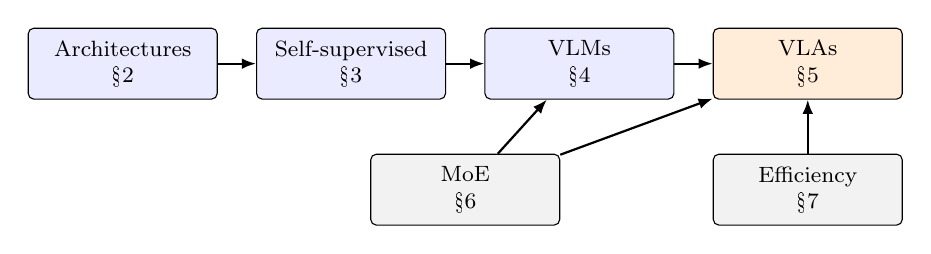
\begin{tikzpicture}[
  box/.style={draw, rounded corners=2pt, align=center, font=\footnotesize, minimum height=9mm, minimum width=24mm, inner sep=3pt},
  arr/.style={-{Latex[length=1.8mm]}, thick}
]
\node[box, fill=blue!8] (a) at (0,0) {Architectures\\\S2};
\node[box, fill=blue!8] (b) at (2.9,0) {Self-supervised\\\S3};
\node[box, fill=blue!8] (c) at (5.8,0) {VLMs\\\S4};
\node[box, fill=orange!15] (d) at (8.7,0) {VLAs\\\S5};
\node[box, fill=gray!10] (e) at (4.35,-1.6) {MoE\\\S6};
\node[box, fill=gray!10] (f) at (8.7,-1.6) {Efficiency\\\S7};
\draw[arr] (a) -- (b); \draw[arr] (b) -- (c); \draw[arr] (c) -- (d);
\draw[arr] (e) -- (c); \draw[arr] (e) -- (d); \draw[arr] (f) -- (d);
\end{tikzpicture}
\caption{The chain this survey follows. Each stage points to a reference implementation (\S8).}
\label{fig:chain}
\end{figure}

\section{Architectures for Perception}

The Transformer~\cite{vaswani2017attention} replaced recurrence with attention. ViT~\cite{dosovitskiy2021vit}
showed that images can be treated as sequences of $16\times16$ patches, DeiT~\cite{touvron2021deit}
made ViTs data-efficient through distillation, and Swin~\cite{liu2021swin} restored the
hierarchy and locality of CNNs with shifted windows. Convolutional backbones remain
competitive: ResNet~\cite{he2016resnet} introduced the residual connection used by every
model in this survey, and ConvNeXt~\cite{liu2022convnext} modernised the ConvNet to match
transformers. For detection, DETR~\cite{carion2020detr} framed the task as set prediction
with bipartite matching, removing hand-designed components such as non-maximum suppression.
Deformable DETR~\cite{zhu2021deformable} attends to a few learned sampling points, which speeds
up convergence. In driving perception, BEVDet~\cite{huang2021bevdet} and BEVFormer~\cite{li2022bevformer}
lift multi-camera features into a bird's-eye-view grid, the latter with spatial
cross-attention and temporal self-attention. Classical multi-view geometry still
underpins all of this: homographies, the direct linear transform and robust estimation
with RANSAC~\cite{hartley2004mvg,fischler1981ransac}.

\section{Self-Supervised Visual Learning}

The central difficulty of self-supervised learning is \emph{collapse}: an encoder that maps
everything to the same vector trivially satisfies any agreement objective. The families
differ mainly in how they prevent it (\cref{tab:ssl}).

\begin{table}[t]
\centering
\caption{Self-supervised families organised by their anti-collapse mechanism.}
\label{tab:ssl}
\small
\begin{tabular}{p{2.8cm}p{4.2cm}p{6.6cm}}
\toprule
Family & Methods & How collapse is avoided \\
\midrule
Contrastive & MoCo~\cite{he2020moco}, SimCLR~\cite{chen2020simclr} & negatives are pushed apart (queue with momentum encoder; large batches) \\
Asymmetric / distillation & BYOL~\cite{grill2020byol}, DINO~\cite{caron2021dino}, DINOv2~\cite{oquab2023dinov2} & predictor head, stop-gradient and momentum teacher; centring and sharpening of teacher outputs \\
Redundancy reduction & Barlow Twins~\cite{zbontar2021barlow}, VICReg~\cite{bardes2022vicreg} & decorrelate embedding dimensions; explicit variance and covariance terms \\
Masked modelling & MAE~\cite{he2022mae} & reconstruct masked input patches (75\% masked), so the target is not the encoder's own output \\
Latent prediction & I-JEPA~\cite{assran2023ijepa}, V-JEPA 2~\cite{assran2025vjepa2} & predict target-encoder \emph{representations} of masked regions with an EMA target \\
\bottomrule
\end{tabular}
\end{table}

For embodied models the JEPA line is especially relevant. Predicting in representation
space rather than pixel space is a world-model objective, and V-JEPA 2~\cite{assran2025vjepa2}
connects video pre-training to action-conditioned prediction and planning.

\section{Vision--Language Models}

Contrastive image--text pre-training (CLIP~\cite{radford2021clip}, and SigLIP~\cite{zhai2023siglip}
with a sigmoid loss) aligns a vision encoder with language. BLIP~\cite{li2022blip} unifies
understanding and generation with caption bootstrapping. LLaVA~\cite{liu2023llava}
established the dominant generative recipe: project patch features from a pretrained
encoder into an LLM's embedding space with a small MLP, then instruction-tune. LoRA~\cite{hu2022lora}
makes the language side cheap to adapt.

\section{Vision--Language--Action Models}

RT-2~\cite{brohan2023rt2} and OpenVLA~\cite{kim2024openvla} treat actions as text tokens of a
fine-tuned VLM. $\pi_0$~\cite{black2024pi0} adds a separate \emph{action expert} trained with flow
matching~\cite{lipman2023flow} to produce continuous action chunks. EO-1~\cite{qu2025eo1}
interleaves vision, text and action during pre-training, and SmolVLA~\cite{shukor2025smolvla}
shows that a compact VLM backbone trained on community data can be competitive. $\pi_{0.5}$~\cite{pi05}
makes four design choices explicit, each a reusable idea:
\begin{enumerate}
  \item \textbf{Action representation.} FAST~\cite{pertsch2025fast} compresses an action chunk with
        a discrete cosine transform followed by byte-pair encoding. Smooth trajectories need
        few coefficients, which makes autoregressive action tokens cheap to \emph{train}. Flow
        matching remains faster at \emph{inference}, because it decodes a chunk in a few
        integration steps rather than token by token.
  \item \textbf{Knowledge insulation.} Stopping gradients from the action expert into the VLM,
        while training the VLM on FAST tokens, preserves the VLM's pretrained knowledge and
        speeds up training~\cite{driess2025ki}.
  \item \textbf{Hierarchy.} A slow ``System 2'' pass of the same VLM decomposes a task into
        subtasks, and a fast ``System 1'' pass produces actions~\cite{shi2025hirobot,pi05}.
  \item \textbf{Real-time chunking.} Treating the next chunk as an inpainting problem
        conditioned on the actions still executing removes discontinuities between chunks
        without retraining~\cite{black2025rtc}.
\end{enumerate}
In practice these separate cleanly: tokenisation for training efficiency, a continuous
expert for inference speed and multi-modality, insulation to protect semantics, and
chunk-level scheduling for smooth control.

\section{Mixture-of-Experts}

Sparsely gated MoE layers~\cite{shazeer2017outrageously} route each token to $k$ of $n$ expert
FFNs. Switch Transformers~\cite{fedus2022switch} simplified routing to $k=1$, and
Mixtral~\cite{jiang2024mixtral} made top-2 MoE mainstream in open models. DeepSeekMoE~\cite{dai2024deepseekmoe}
adds always-on \emph{shared} experts so routed experts can specialise, and DeepSeek-V3~\cite{deepseekv3}
scales this to 671B parameters with 37B active. Sparse activation creates a systems
opportunity as well as a modelling one: only the active experts need to be in fast memory
for any given token.

\section{Efficiency}

\textbf{Training.} FlashAttention~\cite{dao2022flashattention} computes exact attention in tiles
that stay in on-chip SRAM, trading recomputation for far less memory traffic. Mixed
precision~\cite{micikevicius2018mixed} runs most operations in 16-bit with fp32 master weights and
loss scaling. ZeRO~\cite{rajbhandari2020zero} shards optimiser states, gradients and parameters
across data-parallel ranks, and pipeline parallelism~\cite{huang2019gpipe} splits layers across
devices with micro-batching (PyTorch's PiPPy, now \texttt{torch.distributed.pipelining}).
\textbf{Deployment.} Pruning, from magnitude-based pruning within Deep
Compression~\cite{han2016deepcompression} to structured pruning of channels and heads, removes
redundancy, and structured sparsity maps better onto hardware. Integer quantization with
quantization-aware training~\cite{jacob2018quant} recovers accuracy at low bit widths where
post-training quantization degrades.

\section{An Open Ecosystem of Reference Implementations}

\begin{table}[t]
\centering
\caption{Hale/Halo repositories and the survey sections they implement. Facts were verified
against each repository's code (parameter counts measured from the default configurations;
test counts from running the suites on CPU).}
\label{tab:eco}
\small
\begin{tabular}{p{2.5cm}p{6.2cm}p{5.0cm}}
\toprule
Repository & Implements & Verified facts \\
\midrule
Hale-VLA & ViT + MoE decoder VLA with \texttt{<image>}/\texttt{<state>}/\texttt{<action>} tokens (\S2, \S5, \S6) & 355.9M params \\
HALE-WAM & VLA + flow-matching actions + DiT world model (\S5) & 176.3M params \\
Hale-VLM & SigLIP + LoRA on 7--8B LLMs; SmolVLM/SmolVLA data (\S4) & $\approx$72--84M trainable \\
Halo-VLM & pretrained, from-scratch MoE and CLIP-prefix VLMs (\S4, \S6) & 431.5M (scratch MoE) \\
HaleBlocks & shared components, configs, registries, block-causal masks (\S6, \S7) & 114 tests pass \\
HaloBlocks & 37 composable blocks incl.\ MLA, gated attention, MoE (\S2, \S6) & 71 tests pass \\
Hale-LLM & AR vs.\ masked/block diffusion~\cite{sahoo2024mdlm,arriola2025bd3lm} vs.\ flow matching & 47.7M / 63.2M params \\
Hale-Token & MoE experts tiered across unified memory and SSD (\S6, \S7) & logits match \texttt{transformers} \\
\bottomrule
\end{tabular}
\end{table}

\Cref{tab:eco} maps the survey onto the nine repositories (eight code repositories plus this
knowledge base). Each has an arXiv-style write-up, a project page, Mermaid architecture
diagrams, a blog post and agent skills for development. Where the implementations
simplify, for example from-scratch vision encoders instead of SSL-pretrained ones, or
MoE layers without load-balancing losses, the survey's sections indicate what the next
step would be.

\section{Open Questions}

\begin{itemize}
  \item Do routed experts in a VLA specialise by modality (patches, language, action
        queries)? Hale-VLA and Halo-VLM make routing statistics easy to collect.
  \item How much does SSL pre-training (DINOv2~\cite{oquab2023dinov2}, JEPA~\cite{assran2023ijepa})
        of the vision tower improve a small VLA trained on limited robot data, compared with
        training from scratch?
  \item Does predicting future frames (HALE-WAM) improve action prediction, or only
        interpretability, at equal compute?
  \item At small scale, do block diffusion LMs~\cite{arriola2025bd3lm} close the gap to
        autoregressive models on bits per token (Hale-LLM)?
  \item How skewed is expert routing in real workloads, and therefore how much faster than
        the uniform-routing floor is SSD-tiered MoE inference (Hale-Token)?
\end{itemize}

\section{Conclusion}

The path from pixels to robot actions passes through a small number of recurring ideas:
attention over patches, collapse-free self-supervision, projection into language models,
continuous action experts, sparse experts and memory-aware systems. We hope this map, and
the open implementations tied to it, make that path easier to follow.

\bibliographystyle{plainnat}
\bibliography{references}

\end{document}
